\chapter{Top Features by Mutual Information}\label{app:mi}

In this appendix, we report mutual information (\textbf{MI} for short) of features as defined in \Cref{subsubsec:mi}.
We use it for getting the idea of individual features and how to set thresholds for how many features
are used.

Mutual information is a great way to evaluate informativeness of features.
However, it tends to prefer features of higher arity, because
they are more likely to decrease the entropy.
This can be observed in \Cref{tab:mi_words} and \Cref{tab:mi_stars}.


\section{Threshold Features}

First, we report MI of threshold features as listed in \Cref{chap:exp}.
Threshold features cluster instances into groups based on some numeric value.
In the tables bellow, there are features listed with different thresholds.
The meaning of particular thresholds is the following:

\begin{itemize}
\item Features with one threshold are binary --- bellow and above the threshold.
\item \textit{Biz stars} and \textit{stars} are features with five values --- 1 through 5.
\item \textit{Extreme stars} is a yes/no feature expressing whether the number of stars equals 1 or 5.
\item \textit{Review length} with threshold 50, 150 is a ternary feature --- bellow, within and above the interval.
\item \textit{sentiment} is a ternary feature with values negative, neutral and positive.
\end{itemize}

In \Cref{tab:mi_errors}, we report MI of features regarding spelling mistakes.
Feature conveying absolute number of typos has negligible MI, probably owing to the high variance in the reviews' length.
On the contrary, the relative number of typos has proven to be an informative property.
The best performing having MI almost~0.002.

\begin{table}[h!]

\centering
\begin{tabular}{lrS[table-format=3.2]}
\toprule
\textbf{feature} & \textbf{threshold} & \textbf{mutual information} \\
\midrule
error rate & 0.02 & 0.00007 \\
\textbf{error rate} & 0.05 & 0.00182 \\
\textbf{error rate} & 0.10 & 0.00174 \\
error rate & 0.15 & 0.00074 \\
error rate & 0.20 & 0.00038 \\
\midrule
error total & 5 & 0.00000 \\
error total & 10 & 0.00000 \\
error total & 15 & 0.00000 \\
error total & 20 & 0.00000 \\
\bottomrule
\end{tabular}

\caption{Mutual information of spelling mistakes}\label{tab:mi_errors}
\end{table}


The features conveying the number of words turned out to be very informative.
The best performing was the feature with thresholds 50 and 150 having MI 0.07866 which
is more than 40 times more than the best performing error rate.

\begin{table}[h!]

\centering
\begin{tabular}{lrS[table-format=3.2]}
\toprule
\textbf{feature} & \textbf{threshold} & \textbf{mutual information} \\
\midrule
\textbf{review length} & 50, 150 & 0.07866 \\
review length & 35 & 0.02680 \\
review length & 50 & 0.04091 \\
review length & 75 & 0.05996 \\
review length & 100 & 0.06726 \\
review length & 150 & 0.06580 \\

\bottomrule
\end{tabular}
\caption{Mutual information of the number of words}\label{tab:mi_words}
\end{table}

Sentiment has MI approximately 0.01, which is about ten times higher
than error rate, but eight times worse than the number of words.

\begin{table}[h!]
\centering
\begin{tabular}{lrS[table-format=3.2]}
\toprule
\textbf{feature} & \textbf{threshold} & \textbf{mutual information} \\
\midrule
sentiment & neg, neut, pos & 0.00969 \\
\bottomrule
\end{tabular}
\caption{Mutual information of sentiment}\label{tab:mi_sentiment}
\end{table}

It follows from the experiments, that it greatly depends what instances
we choose for the cosine similarity features.
Only two out of ten instances in the cosine similarity corpus resulted in
non-negligible MI.
The best performing instances has MI of~\num{0.00006}, which is insignificant
in comparison with other features.

\begin{table}[h!]
\centering
\begin{tabular}{lrS[table-format=3.2]}
\toprule
\textbf{feature} & \textbf{threshold} & \textbf{mutual information} \\
\midrule
\textbf{instance 1} & 0.40 & 0.00006 \\
instance 1 & 0.60 & 0.00002 \\
instance 1 & 0.80 & 0.00002 \\
instance 1 & 0.90 & 0.00002 \\
instance 1 & 0.95 & 0.00002 \\
\midrule
\textbf{instance 2} & 0.40 & 0.00004 \\
instance 2 & 0.60 & 0.00002 \\
instance 2 & 0.80 & 0.00002 \\
instance 2 & 0.90 & 0.00002 \\
instance 2 & 0.95 & 0.00002 \\
\bottomrule
\end{tabular}
\caption{Mutual information of cosine similarity (2 best performing instances)}\label{tab:mi_cossim}
\end{table}

The best performing feature for stars convey the exact number of stars.
It has MI 0.01, which is comparable to sentiment.

The second best feature, \textit{whether the number of stars equals one}, shows a disadvantage of mutual information as a metrics for evaluate goodness of features.

The MI is fairly high and the feature looks useful at first.
Reviews giving only one star are likely to express serious complains, which are probably more useful than praising a business.
Data analysis backs this claim --- approximately 78\% of 1 star reviews have been repeatedly marked as useful.
However, the problem is that there is only as much as 0.4\% reviews giving 1 star making this
feature virtually worthless.

\begin{table}[h!]
\centering
\begin{tabular}{lrS[table-format=3.2]}
\toprule
\textbf{feature} & \textbf{threshold} & \textbf{mutual information} \\
\midrule
biz stars & 1, 2, 3, 4, 5 & 0.00112 \\
extreme stars & 1, 5 & 0.00175 \\
\textbf{stars} & 1, 2, 3, 4, 5& 0.01060 \\
stars & 1 & 0.00657 \\
stars & 2 & 0.00204 \\
stars & 3 & 0.00221 \\
stars & 4 & 0.00137 \\
stars & 5 & 0.00004 \\
\bottomrule
\end{tabular}

\caption{Mutual information of stars}\label{tab:mi_stars}
\end{table}


\section{Existential Features}

Second, we report mutual information of existential features.
Those features express whether a certain phrase exist in the text.

The value of the function in the two graphs bellow expresses
MI of the~$x$-th best feature at the point~$x$.
It is the same as if we ordered the feature in the descending order
and plotted their MI in the order.
Note that x axis is logarithmic.

In \Cref{fig:mi_unigrams},
we can see that only top 1000 performing unigrams have non-negligible MI.
\Cref{fig:mi_entities} expresses the same for entities
--- approximately 1000 features are somewhat informative.


\begin{figure}[ht]\centering
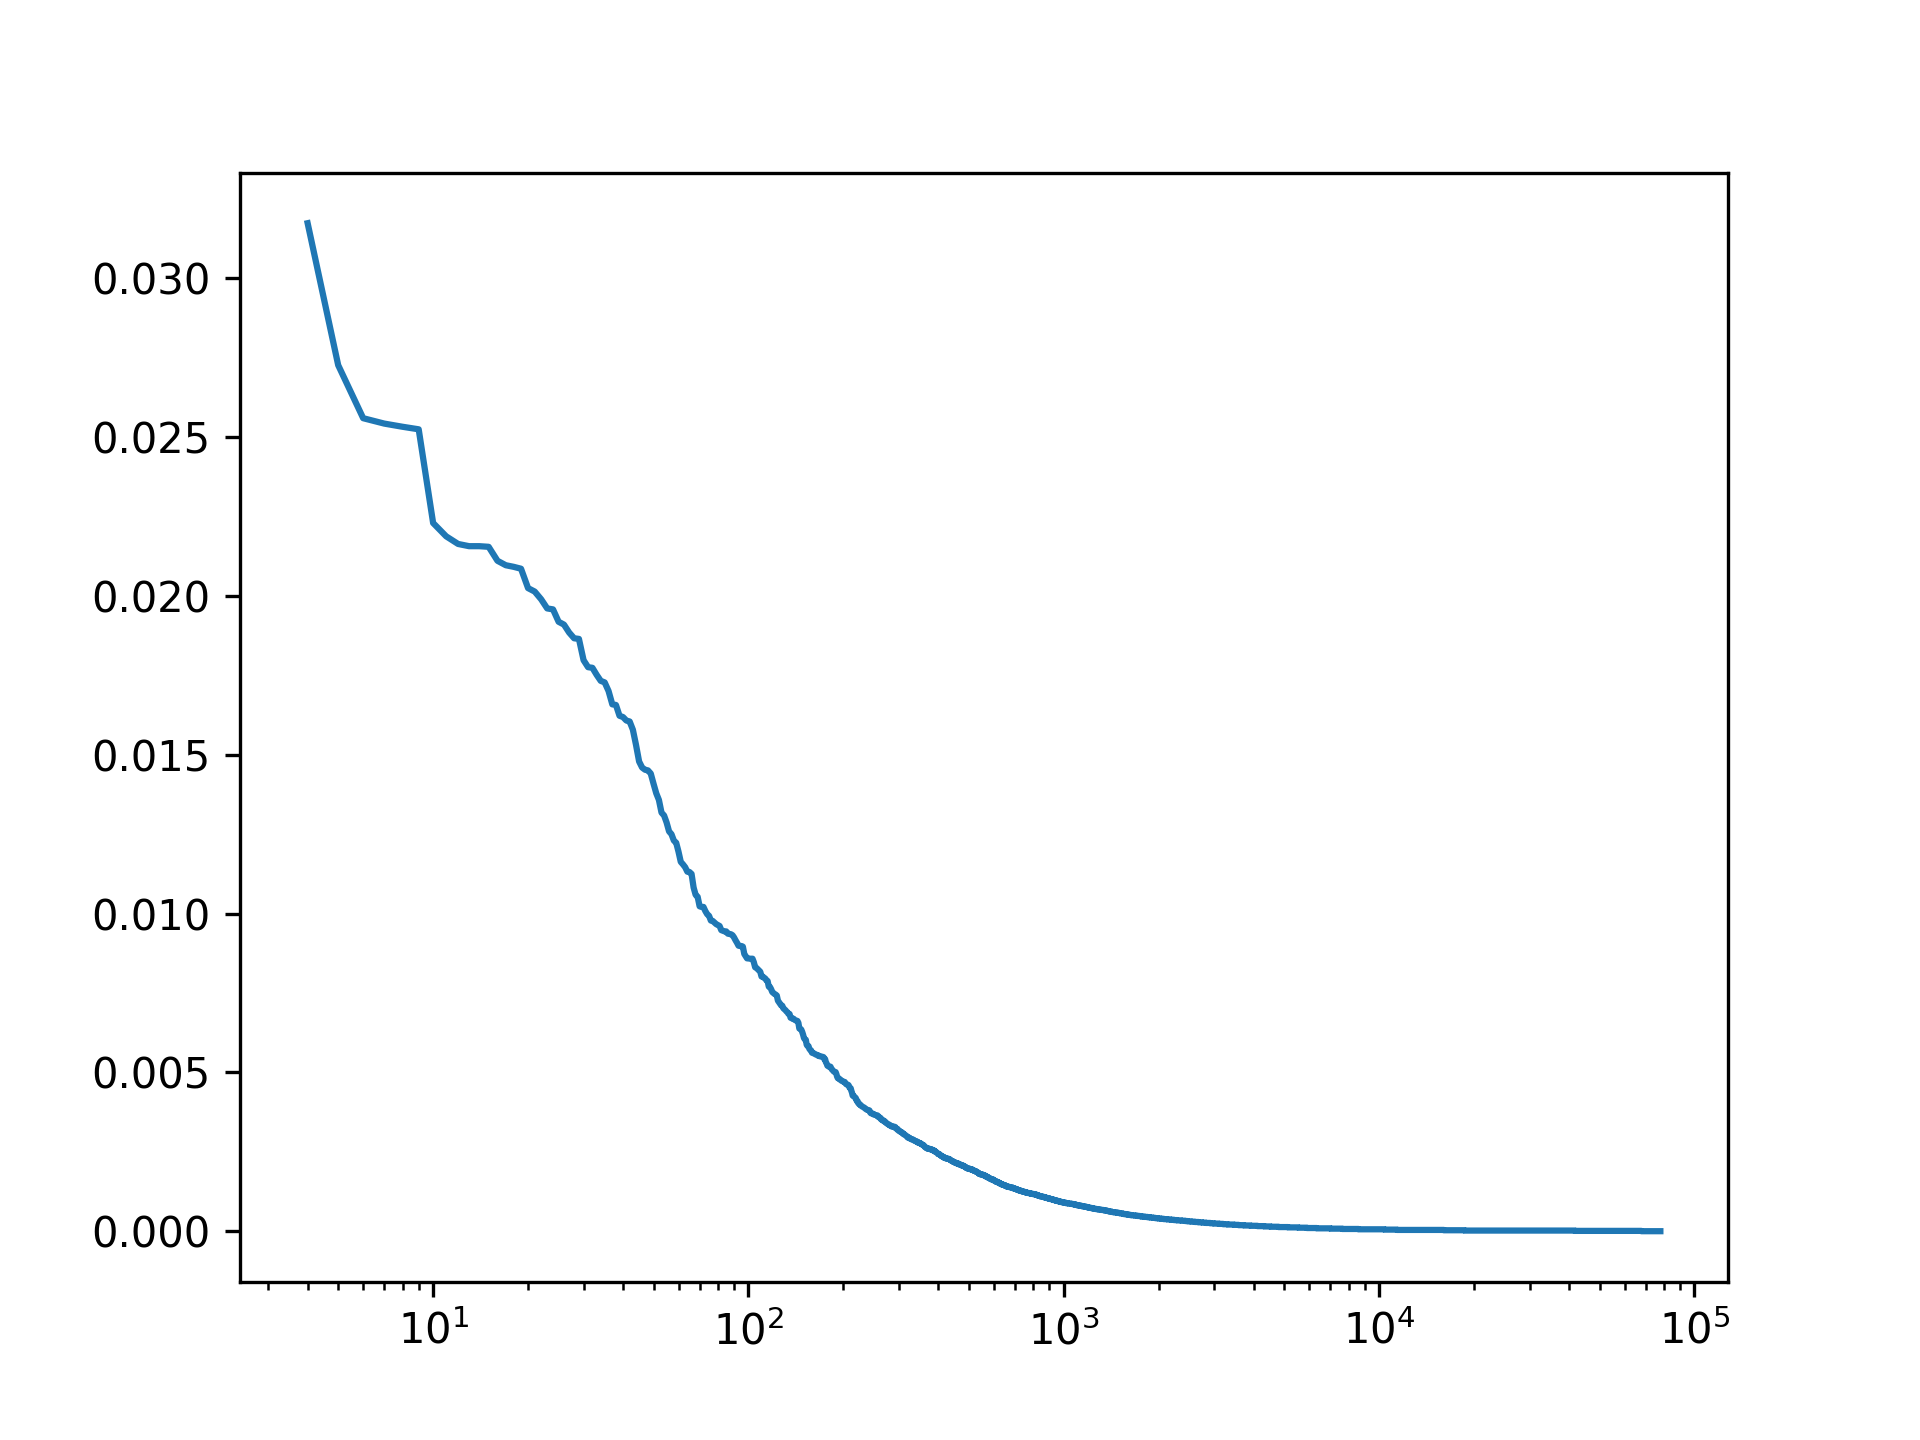
\includegraphics[width=130mm]{figures/unigrams.png}
\caption{Mutual information of unigrams}
\label{fig:mi_unigrams}
\end{figure}


\begin{figure}[ht]\centering
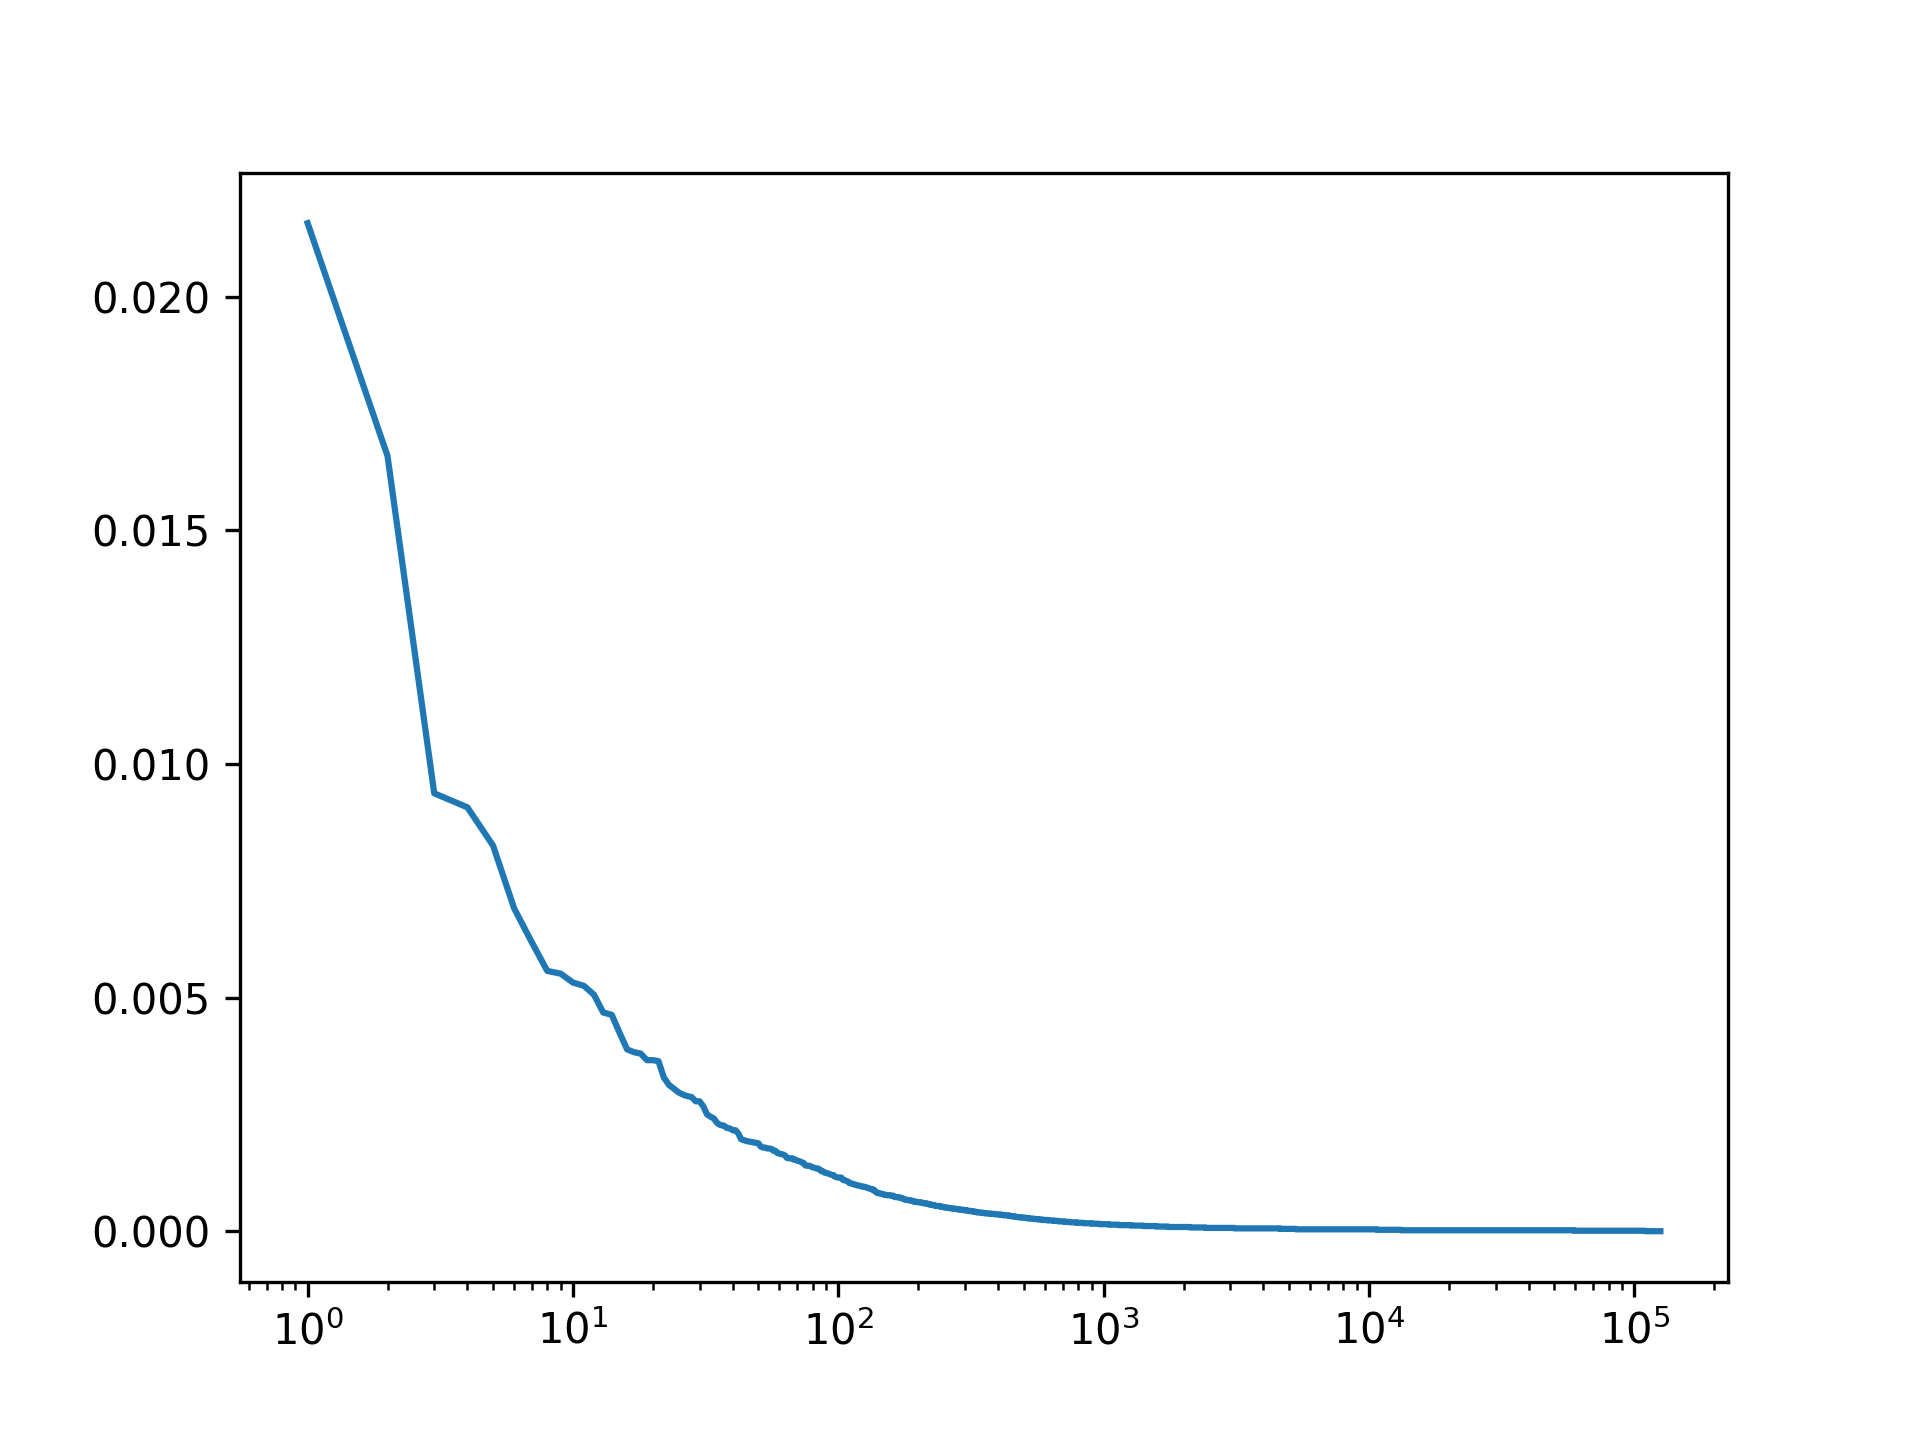
\includegraphics[width=130mm]{figures/entities.png}
\caption{Mutual information of entities}
\label{fig:mi_entities}
\end{figure}
